%****************************************************************************%
%* DIET User's Manual Performance prediction chapter file                   *%
%*                                                                          *%
%*  Author(s):                                                              *%
%*    - Martin QUINSON (Martin.Quinson@loria.fr) (FAST)                     *%
%*    - Peter FRAUENKRON (Peter.Frauenkron@gmail.com) (CoRI)                *%
%*                                                                          *%
%* $LICENSE$                                                                *%
%****************************************************************************%

\chapter{Performance prediction}
\label{chapter:performance}
\section{Introduction}

As we have seen in Chapter~\ref{ch:plugin} the agent needs some
information from the \sed to make an optimal scheduling. This
information is a performance prediction of the \sed. The agent will ask
the \sed to fill the data structure defined in Chapter~\ref{ch:plugin}
with the information it needs. The \sed returns the information and the
agent can make the scheduling. \\ Performance prediction can be based
on hardware information, the charge of the \sed (the charge of the CPU,
of the memory,...) or an advanced performance prediction can combine
a set of basic performance predictions. It is possible to use FAST in
the plug-in scheduler to obtain advanced performance predictions. A
second possibility to get performance prediction, called CoRI, is now
available.  The aim of CoRI is to simplify the access to the
information. Inside of CoRI, FAST can be called, but it is only one
source of information among other sources (for example Cori-Easy). \\
FAST is described in Section~\ref{sec:FAST}, CoRI is described in
Section~\ref{sec:CORI}.\\ The default compiling is without FAST and
without CoRI. Note that if you compile with batch enabled, then CoRI
is also enabled.  In the table~\ref{t:depcompil} you can see which
information is available with each compiling option.

\begin{table}[h]
 \tiny
 \centering
 \begin{tabular}[c]{|l|c|c||c||c|}\hline
%Cori ligne
   &
  \multicolumn{4}{|c|}{\textbf{-DDIET\_USE\_CORI:}} \\[5pt]
   &
  \multicolumn{2}{|c||}{\textbf{BOOL=OFF}} &
  \multicolumn{2}{|c|}{\textbf{BOOL=ON}}\\[5pt]
  \hline
  \hline
%FAST ligne

  \texttt{Information tag} 
  & \multicolumn{4}{|c|}{\textbf{-DDIET\_USE\_FAST:}} \\[5pt]
 \texttt{starts with EST\_} & BOOL=OFF & BOOL=ON  & BOOL=OFF & BOOL=ON \\[5pt]
  \hline

%TAGS lines
 \textit{TCOMP        }      &   & x &   &    \\[5pt]
 \hline 
%  \textit{TIMESINCELASTSOLVE} & x & x & x & x  \\[5pt]
%  \hline
  \textit{FREECPU      }      &   & x & x & x  \\[5pt]
  \hline
  \textit{FREEMEM      }      &   & x & x & x  \\[5pt]
  \hline
  \textit{NBCPU        }      &   & x & x & x  \\[5pt]
  \hline
  \textit{CPUSPEED     }      &   &   & x & x  \\[5pt]
  \hline
  \textit{TOTALMEM     }      &   &   & x & x  \\[5pt]
  \hline
  \textit{AVGFREECPU   }      &   &   & x & x  \\[5pt]
  \hline
  \textit{BOGOMIPS     }      &   &   & x & x  \\[5pt]
  \hline
  \textit{CACHECPU     }      &   &   & x & x  \\[5pt]
  \hline
  \textit{TOTALSIZEDISK}      &   &   & x & x  \\[5pt]
  \hline
  \textit{FREESIZEDISK }      &   &   & x & x  \\[5pt]
  \hline
  \textit{DISKACCESREAD}      &   &   & x & x  \\[5pt]
  \hline
  \textit{DISKACCESWRITE}     &   &   & x & x  \\[5pt]
  \hline
  \textit{ALLINFOS     }      &   &   & x & x  \\[5pt]
  \hline
  \hline
  & \multicolumn{4}{|c|}{\textbf{-DDIET\_USE\_BATCH=ON}} \\[5pt]  
  \textit{PARAL\_NB\_FREE\_RESOURCES\_IN\_DEFAULT\_QUEUE} & & & x & x  \\[5pt] 
  \hline
 \end{tabular}
 \caption{Dependencies of the available information on the
 compiling options}
 \label{t:depcompil}
\end{table}

%====[ FAST: FAST AGENT'S SYSTEM TIMER ]=======================================
\section{FAST: Fast Agent's System Timer}
\label{sec:FAST}

This section deals with FAST, a performance prediction module that can
be used by \diet. It is non-mandatory, but can provide {\sed}s with
improved performance prediction capability.\\
You can use FAST in stand-alone mode without having compiled with
CoRI option.

FAST~\cite{Qui02} is a tool for dynamic performance forecasting in a
Grid environment. As shown in Figure~\ref{fig:fast-overview}, FAST
is composed of several layers and relies on a variety of low-level
software. First, it uses the Network Weather Service
(NWS)~\cite{WSH99}, a distributed system that periodically monitors
and dynamically forecasts the performances of various network and
computational resources. The resource availabilities acquisition
module of FAST uses and enhances NWS. Indeed, if there is no direct
NWS monitoring between two machines, FAST automatically searches for
the shortest path between them in the graph of monitored links. It
estimates the bandwidth as the minimum of those in the path and the
latency as the sum of those measured. This allows the
availability of more predictions when \diet is deployed over a
hierarchical network.

\begin{figure}[htb]
  \begin{center}
    \includegraphics[scale=0.75]{fig/FAST}
    \caption{FAST overview}
    \label{fig:fast-overview}
  \end{center}
\end{figure}

In addition to system availabilities, FAST can also forecast the
time and space needs of certain computational routines as a function
of the problem parameters and the machines where the computations
would take place.  FAST is particularly suited to numerical algebra
routines whose performance is not data-dependent and where a clear
relationship exists between problem size and performance. As a basis
for predictions, FAST benchmarks the routines at installation time
on each machine for a representative set of parameters. After
polynomial data fitting, the results are stored in an LDAP tree. The
user API of FAST is composed of a small set of functions that
combine resource availabilities and routine needs from low-level
software to produce ready-to-use values.  These results can be
combined into analytical models by the parallel
extension~\cite{CS02} to forecast execution times of parallel
routines.

FAST clients can access information like the time needed to move a
given amount of data between two FAST-enabled machines {\sed}s, the
time to solve a problem with a given set of computational resources,
or the combination of these two quantities.\\

For more details about FAST, please refer to the FAST
webpage~\footnote{\url{http://www.loria.fr/~quinson/fast.html}}.
% the FAST Reference Manual~\footnote{\url{http://graal.ens-lyon.fr/FAST/docs}}.

\subsection{Building FAST}

The first step is to download and install FAST and its
dependent programs.  FAST depends on:
\begin{itemize}
 \item{\textbf{NWS}} the Network Weather Service
 \item{\textbf{GSL}} the GNU Scientific Library
 \item{\textbf{OpenLDAP}} an implementation of the Lightweight
                          Directory Access Protocol
\end{itemize}
Of course, you also need to install the FAST SDK itself. It is important to
 basically understand how FAST works, and the role of its dependencies, to
deactivate the ones that are not needed by the user.

\subsection{Using FAST in the plug-in scheduler}\label{subsection:callFAST}

FAST- and NWS-based performance estimation metrics are stored in
  an estimation metric vector (see Chapter~\ref{ch:plugin} for more details) by calling
  \begin{tabbing}
    \texttt{int diet\_estimate\_fast(}\=\texttt{estVector\_t ev,} \\
    \> \texttt{const diet\_profile\_t* const profilePtr)};
  \end{tabbing}
   with an appropriate value for \texttt{ev} and the
   \texttt{profilePtr} corresponding to the current \diet request.

   \textbf{Attention: } this option it not available when compiling 
   with the option \texttt{-DDIET\_USE\_CORI} set to \texttt{OFF}, 
   To access to this information use CoRI.
   (see Section~\ref{sec:CORI}).

\subsection{Building a server application with FAST}

Since performance prediction is performed only in the \diet \sed,
no modification is needed to the client code.

On the other hand, at the \sed-level the code must sometimes be adapted.  In
the next subsection we explain convertors and show how they can be used
in an example.

\subsubsection{Using convertors}

The service profiles offered by \diet are sometimes not
understandable by the service implementations. To solve this problem,
a convertor processes each profile before it is passed to the
implementation. This is mainly used to
hide the implementation specific profile of a service from
the user. It allows different servers to declare the same
service with the same profile using different implementations
of the service. As FAST relies on the path of the service, the
convertor can also change the path of the declared profile to
enable a correct evaluation of the incoming requests by FAST.
If no convertor is passed when declaring a new service, a
default convertor is assigned to it that does not change its
profile nor its path.

To translate a profile, the convertor defines a new
destination profile with a new path. It then chooses for
each argument of the new profile a predefined function
to assign this argument from the source profile. This
allows the following operations:

\begin{description}
\item{\textbf{Permutation of arguments}}. This is done implicitly by
  specifying which argument in the source profile corresponds to which
  argument in the destination profile.
\item{\textbf{Copy of arguments}}. Arguments can be simply used by
  applying the \texttt{DIET\_CVT\_IDENTITY} function. If the same
  source argument corresponds to two destination arguments it is
  automatically copied.
\item{\textbf{Creation of new arguments}}. New arguments can either
  contain static values or the properties of existing arguments. To
  create a new static value, the index for the source argument must be
  invalid (e.g. -1) and the arg parameter must be set to the static
  argument. To extract a property of an existing argument, other
  functions than \texttt{DIET\_CVT\_IDENTITY} must be applied. The
  result of this function will then be used as the value for the
  destination argument.  Corresponding to the \diet datatypes, the
  following functions exist: \\
\begin{itemize}
\item{\texttt{DIET\_CVT\_IDENTITY}} Copy the argument
\item{\texttt{DIET\_CVT\_VECT\_SIZE}} Get the size of a vector
\item{\texttt{DIET\_CVT\_MAT\_NB\_ROW}} Get the number of rows of a matrix
\item{\texttt{DIET\_CVT\_MAT\_NB\_COL}} Get the number of columns of a matrix
\item{\texttt{DIET\_CVT\_MAT\_ORDER}} Get the order of a matrix
\item{\texttt{DIET\_CVT\_STR\_LEN}} Get the length of the string
\item{\texttt{DIET\_CVT\_FILE\_SIZE}} Get the size of the file
\end{itemize}
Only the \texttt{DIET\_CVT\_IDENTITY} function can be applied to any
argument; all other functions only operate on one type of argument.

\end{description}

\subsection{Example with convertors}

\noindent A short example is available below:
\footnotesize
\begin{verbatim}

/**
 * Example 1
 * Assume we declared a profile (INOUT MATRIX) with the path 'solve_T'.
 * This profile will be called by the client. Our implementation expects
 * a profile (IN INT, IN INT, INOUT MATRIX). This profile is known to
 * FAST with the path 'T_solve'.
 * We will write a convertor that changes the name and extracts the
 * matrix's dimensions.
 */
    // declare a new convertor with 2 IN, 1 INOUT and 0 OUT arguments
    cvt = diet_convertor_alloc("T_solve", 0, 1, 1);

    // apply the function DIET_CVT_MAT_NB_ROW to determine the
    // 0th argument of the converted profile. The function's
    // argument is the 0th argument of the source profile. As it
    // is an IN argument, the last parameter is not important.
    diet_arg_cvt_set(&(cvt->arg_convs[0]), DIET_CVT_MAT_NB_ROW, 0, NULL, 0);

    // apply the function DIET_CVT_MAT_NB_COL to determine the
    // 1st argument of the converted profile. The function's
    // argument is the 0th argument of the source profile. As it
    // is a IN argument, the last parameter is not important.
    diet_arg_cvt_set(&(cvt->arg_convs[1]), DIET_CVT_MAT_NB_COL, 0, NULL, 0);

    // apply the function DIET_CVT_IDENTITY to determine the
    // 2nd argument of the converted profile. The function's
    // argument is the 0th argument of the source profile and
    // it will be written back to the 0th argument of the source
    // profile when the call has finished.
    diet_arg-cvt_set(&(cvt->arg_convs[2]), DIET_CVT_IDENTITY, 0, NULL, 0);

    // NOTE: The last line could also be written as:
    //diet_arg_cvt_short_set(&(cvt->arg_convs[2]), 0, NULL);

    // add the service using our convertor
    diet_service_table_add(profile, cvt, solve_T);

    // free our convertor
    diet_convertor_free(cvt);
\end{verbatim}
\normalsize

\noindent More examples on how to create and use convertors are given in the
files \\
\texttt{examples/dmat\_manips/server.c} and \texttt{examples/BLAS/server.c}.

\section{CoRI: Collectors of Ressource Information}
\label{sec:CORI}

CoRI manages the access to different tools for collecting information
about the \sed. At present, three tools, called collectors, are
implemented: FAST, CoRI Easy and CoRI batch. The user can choose which
collector will provide the information.

\begin{figure}[h]
  \begin{center}
    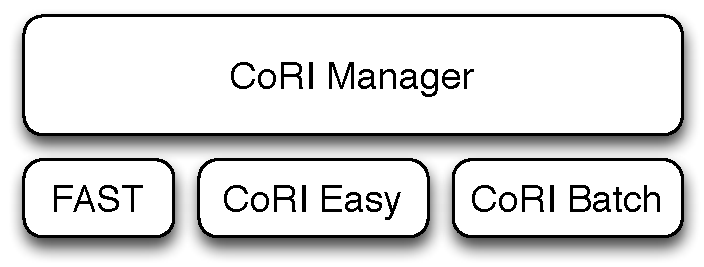
\includegraphics[scale=0.5]{fig/overviewCori}
    \caption{CoRI overview}
    \label{fig:cori-overview}
  \end{center}
\end{figure}

\subsection{Functions and tags}
The tags for information are of type \texttt{integer} and defined in
the table~\ref{t:tags}. The second type of tag
\texttt{diet\_est\_collect\_tag\_t} is used to specify which collector
will provide the information: \texttt{EST\_COLL\_FAST},
\texttt{EST\_COLL\_EASY} or \texttt{EST\_COLL\_BATCH}. Three different
functions are provided with CoRI.

The first function initializes a specific collector.

\footnotesize
\begin{verbatim}
  int
  diet_estimate_cori_add_collector(diet_est_collect_tag_t collector_type,
                                   void * data);
\end{verbatim}
\normalsize The second parameter is reserved for initializing
collectors which need additional information on initialization. For
example, the BATCH collector needs for its initialization the profile
of the service to be solved.

After the initialization, accessing to the information is done by
specifying the collector and the information type. 
\footnotesize
\begin{verbatim}
  int
  diet_estimate_cori(estVector_t ev,
                     int info_type,
                     diet_est_collect_tag_t collector_type,
                     void* data);
\end{verbatim}
\normalsize

Cori-Easy doesn't need more information, but FAST and BATCH need a
profile of type ``diet\_profile\_t''. The last parameter is reserved
for it. \\ The last function is used to test Cori-Easy. It prints all
information Cori-Easy finds to the standard output.

\footnotesize
\begin{verbatim}
  void
  diet_estimate_coriEasy_print();
\end{verbatim}
\normalsize
A result could be the following output:
\footnotesize
\begin{verbatim}
start printing CoRI values..
cpu average load : 0.56
CPU 0 cache : 1024 Kb
number of processors : 1
CPU 0 Bogomips : 5554.17
diskspeed in reading : 9.66665 Mbyte/s
diskspeed in writing : 3.38776 Mbyte/s
total disk size : 7875.51 Mb
available disk size  :373.727 Mb
total memory : 1011.86 Mb
available memory : 22.5195 Mb
end printing CoRI values
\end{verbatim}
\normalsize

\subsection{FAST}
FAST as collector of CoRI gives the user the same information as
without CoRI, see table~\ref{t:depcompil} to know which information FAST can
provide.

\subsection{CoRI-Easy}
The CoRI-Easy collector makes some basic system calls to gather the
information. CoRI-Easy is only available if \diet is compiled with the
option \texttt{-DDIET\_USE\_CORI} set to \texttt{ON}. The last collumn
of the table~\ref{t:depcompil} corresponds to the CoRI-Easy's
functionality.

There is an example on how to use CoRI-Easy in the
\verb!<diet_src>/src/examples/cori/! directory.

\subsection{CoRI batch}\label{section:cori_batch}
With the help of the CoRI batch collector, a \sed programmer can use
some information obtained from the batch system. It is only available
if \diet is compiled with the option \texttt{-DDIET\_USE\_BATCH} set
to \texttt{ON}. For the moment, only simple information can be
accessed but functionalities will be improved as well as the number of
recognizable batch systems.

There is an example on how to use CoRI batch in the\\
\verb!<diet_src>/src/examples/Batch/SparseSolver/! directory.

\section{Future Work}

There are two primary efforts for the CoRI manager:
\begin{itemize}
\item \textbf{Improving CoRI-Easy}: Some evaluation functions are very
  basic and should be revised to increase their response time speed
  and the accuracy of the information.  There is a need for other
  information (i.e. information about the network).  Every operating
  systems provide other basic functions to get the information.
  CoRI-Easy doesn't know all functions. Use the
  \texttt{diet\_estimate\_cori\_print()} function to test what
  CoRI-Easy can find on your \sed. Send us a mail if not  all functions
  are working properly.

\item \textbf{Improving CoRI batch}: add new functionalities to access
dynamic information as well as some kind of performance predictions
for more batch systems.

\item \textbf{New collectors}: Integrating other external tools like
  Ganglia~\cite{Ganglia} or Nagios~\cite{Nagios} to the CoRI Manager
  can provide more useful and exact information.
\end{itemize}

%%% Local Variables:
%%% mode: latex
%%% ispell-local-dictionary: "american"
%%% mode: flyspell
%%% fill-column: 79
%%% End:
